\section{Bases de datos}

\subsection{Conjuntos de entrenamiento y pruebas}
Los valores conocidos de la matriz $M$ se dividen en dos subconjuntos: de entrenamiento y de prueba. El conjunto de entrenamiento se utiliza para predecir los valores que no se conocen, mientras que el conjunto de prueba se utiliza para evaluar el desempeño de cada método.

Usualmente se utilizará un $80\%$ de los datos conocidos en el conjunto de entrenamiento y un $20\%$ en el conjunto de prueba. Estos dos conjuntos no necesariamente van a ser disjuntos.

\subsection{Netflix\_3m1k}
Esta será la principal base de datos con la que vamos a hacer pruebas. Consiste en 4427 usuarios, 1000 items y 56136 clasificaciones, es decir, una densidad del 1.27 \%. Las clasificaciones están distribuidas como se muestra en la figura~\ref{fig:netflix_data_distribution}. Podemos observar que la mayoría de las clasificaciones son 3, 4, o 5. De lo anterior, podríamos interpretar que las personas solo califican las películas que sí les gustaron, en otro caso prefieren no dar una calificación en lugar de dar una muy baja.

Luego, en las figuras~\ref{fig:means_and_vars_by_row}~y~\ref{fig:means_and_vars_by_col} se observan las distribuciones de medias y varianzas por filas y columnas, respectivamente. Notemos que tanto en filas como columnas hay picos en los números enteros y muchas varianzas con valor cero. Con eso podemos decir que muchas de las personas siempre dieron la misma calificación a todas las películas que han visto.

% \begin{table}[h]
%     \centering
%     \caption{Bases de datos}
%     \begin{tabular}{|l|c|c|c|c|}
%         \hline
%         Base de datos & Usuarios & Items & Clasificaciones & Densidad \\ \hline 
%         Netflix3m1k & 4427 & 1000 & 56136 & 1.27 \% \\\hline
%     \end{tabular}
% \end{table}

\begin{figure}[ht]
    \centering
    \includegraphics[width=0.4\linewidth]{../Results/Netflix/Plots/Data_distribution.png}
    \caption{Distribución de clasificaciones en Netflix\_3m1k}\label{fig:netflix_data_distribution}
\end{figure}

\begin{figure}[ht]
    \centering
    \subfigure[Medias]{\includegraphics[width=0.4\linewidth]{../Results/Netflix/Plots/Hist_Mean_Rows.png}}
    \subfigure[Varianzas]{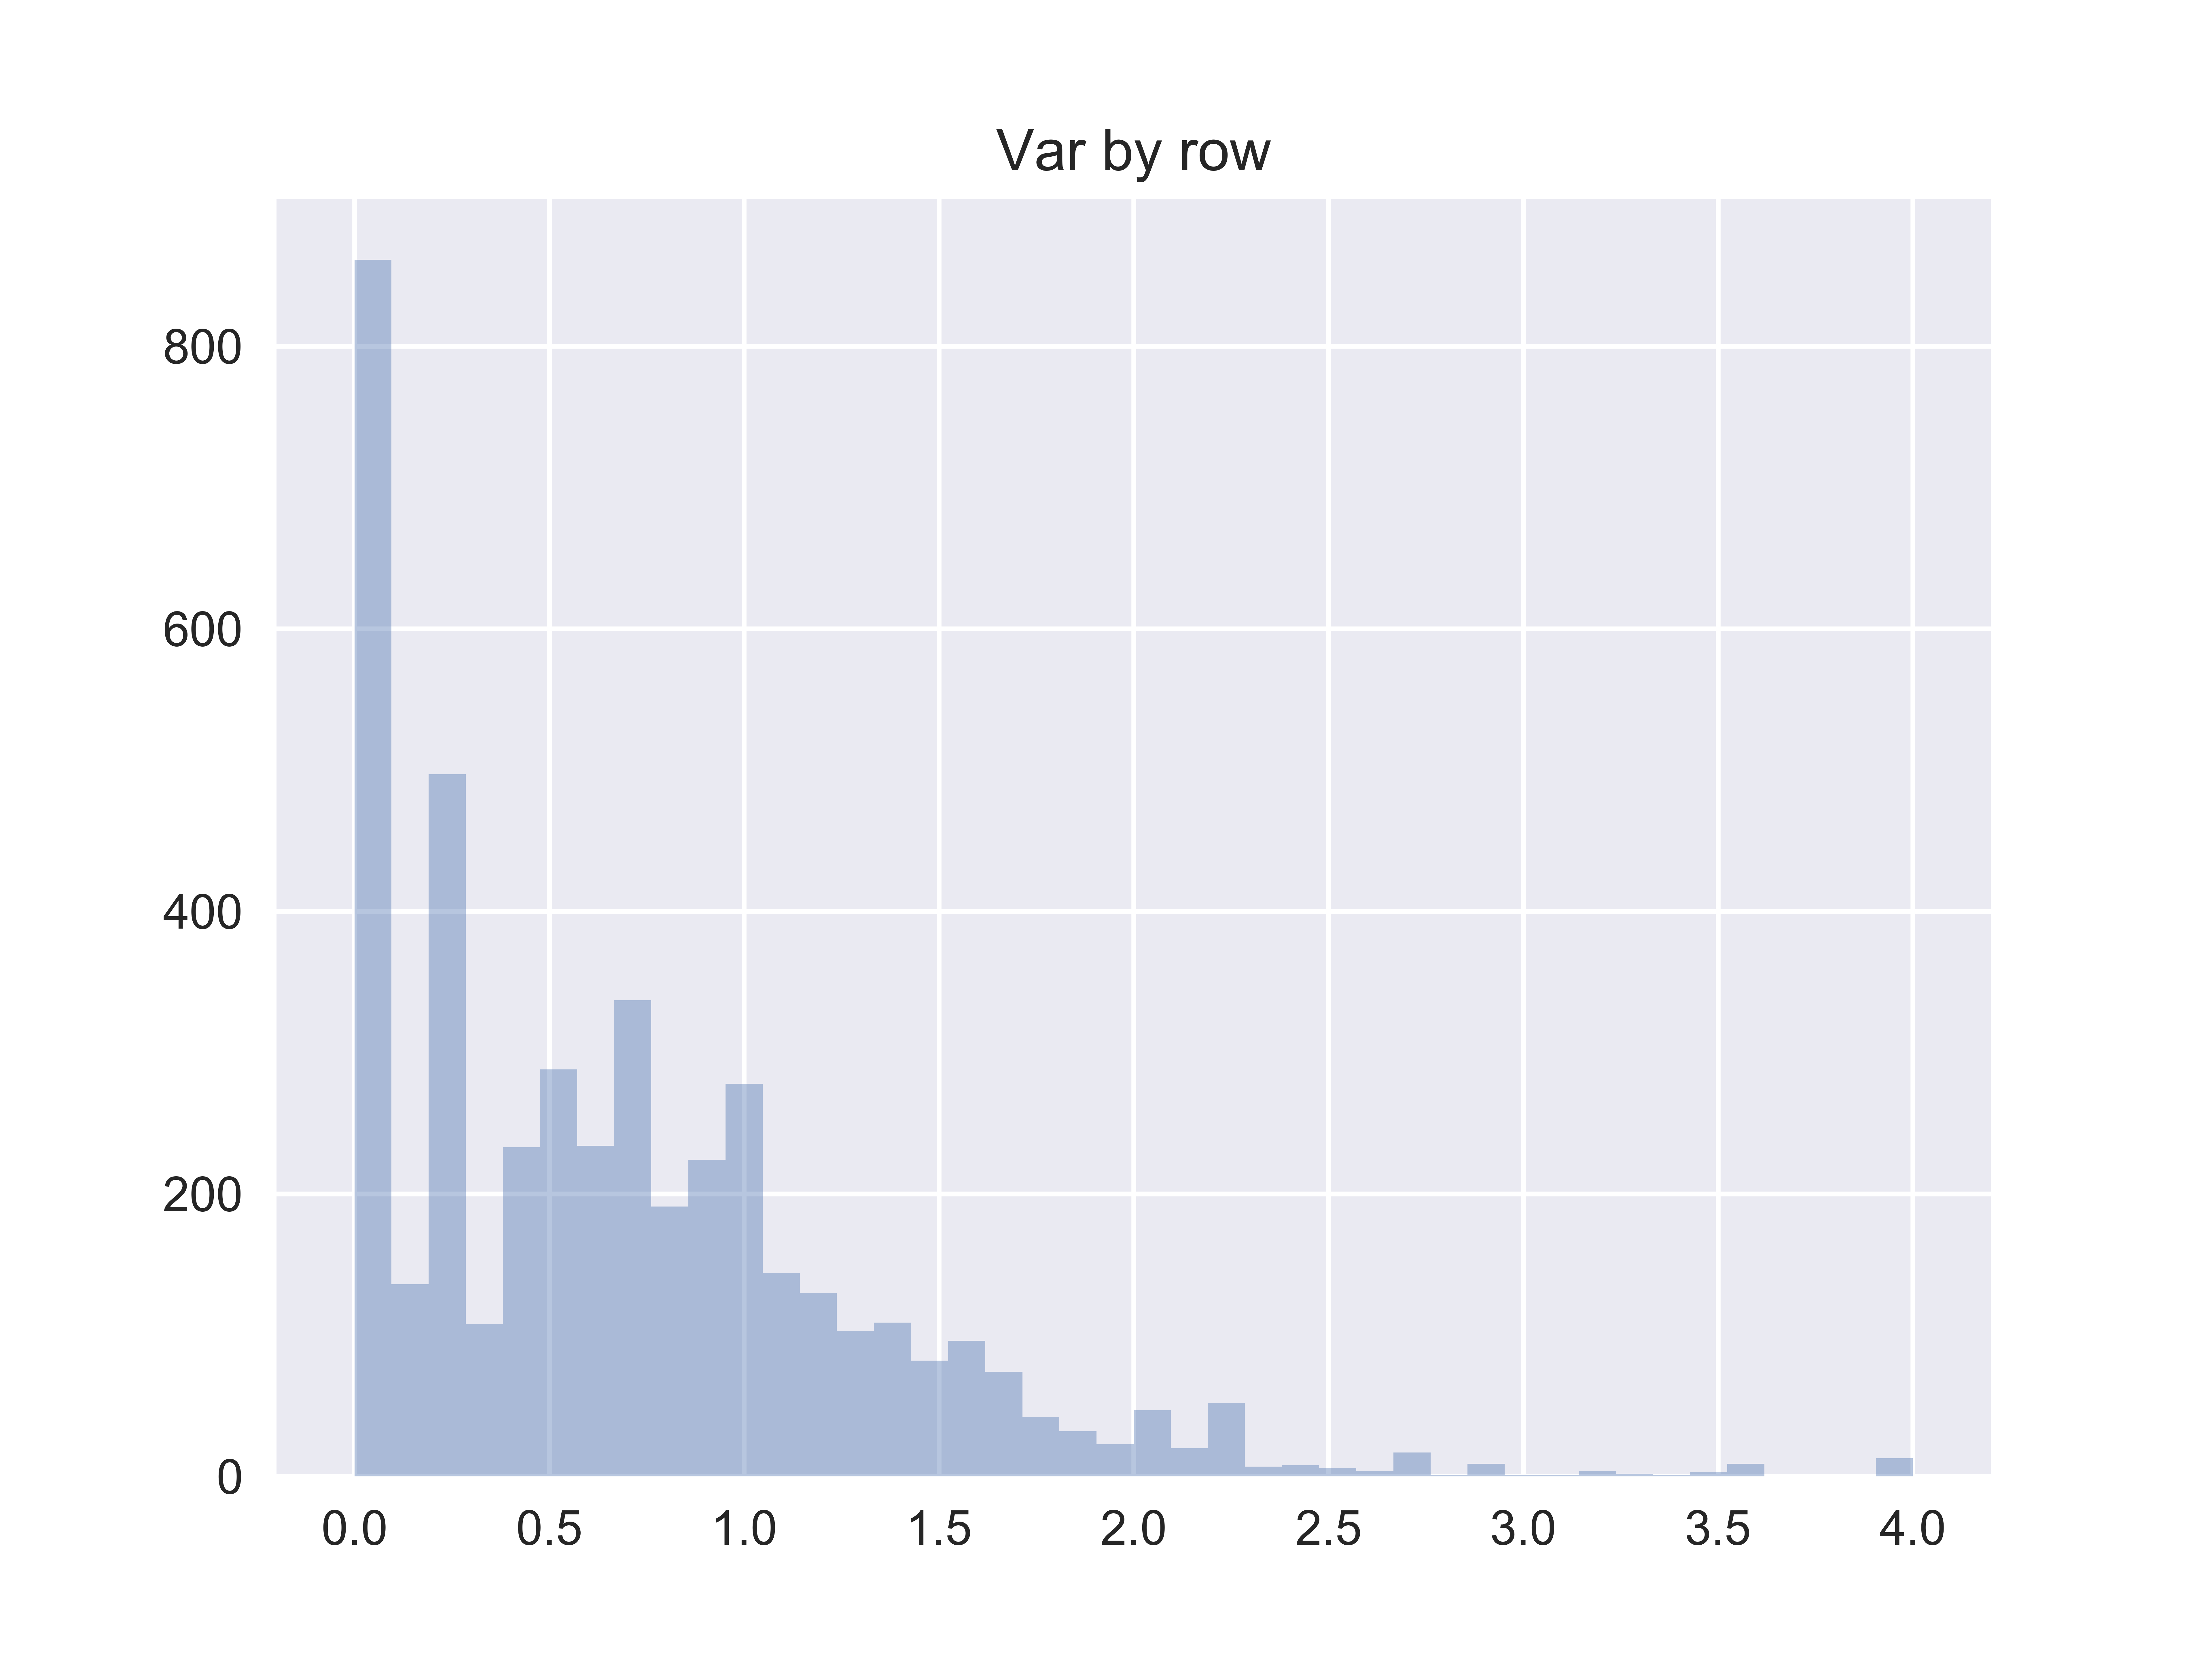
\includegraphics[width=0.4\linewidth]{../Results/Netflix/Plots/Hist_Var_Rows.png}}
    \caption{Medias y varianzas por filas}\label{fig:means_and_vars_by_row}
\end{figure}

\begin{figure}[ht]
    \centering
    \subfigure[Medias]{\includegraphics[width=0.4\linewidth]{../Results/Netflix/Plots/Hist_Mean_Cols.png}}
    \subfigure[Varianzas]{\includegraphics[width=0.4\linewidth]{../Results/Netflix/Plots/Hist_Var_Cols.png}}
    \caption{Medias y varianzas por columnas}\label{fig:means_and_vars_by_col}
\end{figure}

% \begin{figure}[htb]
%     \centering
%     \subfigure[Por número de vecinos]{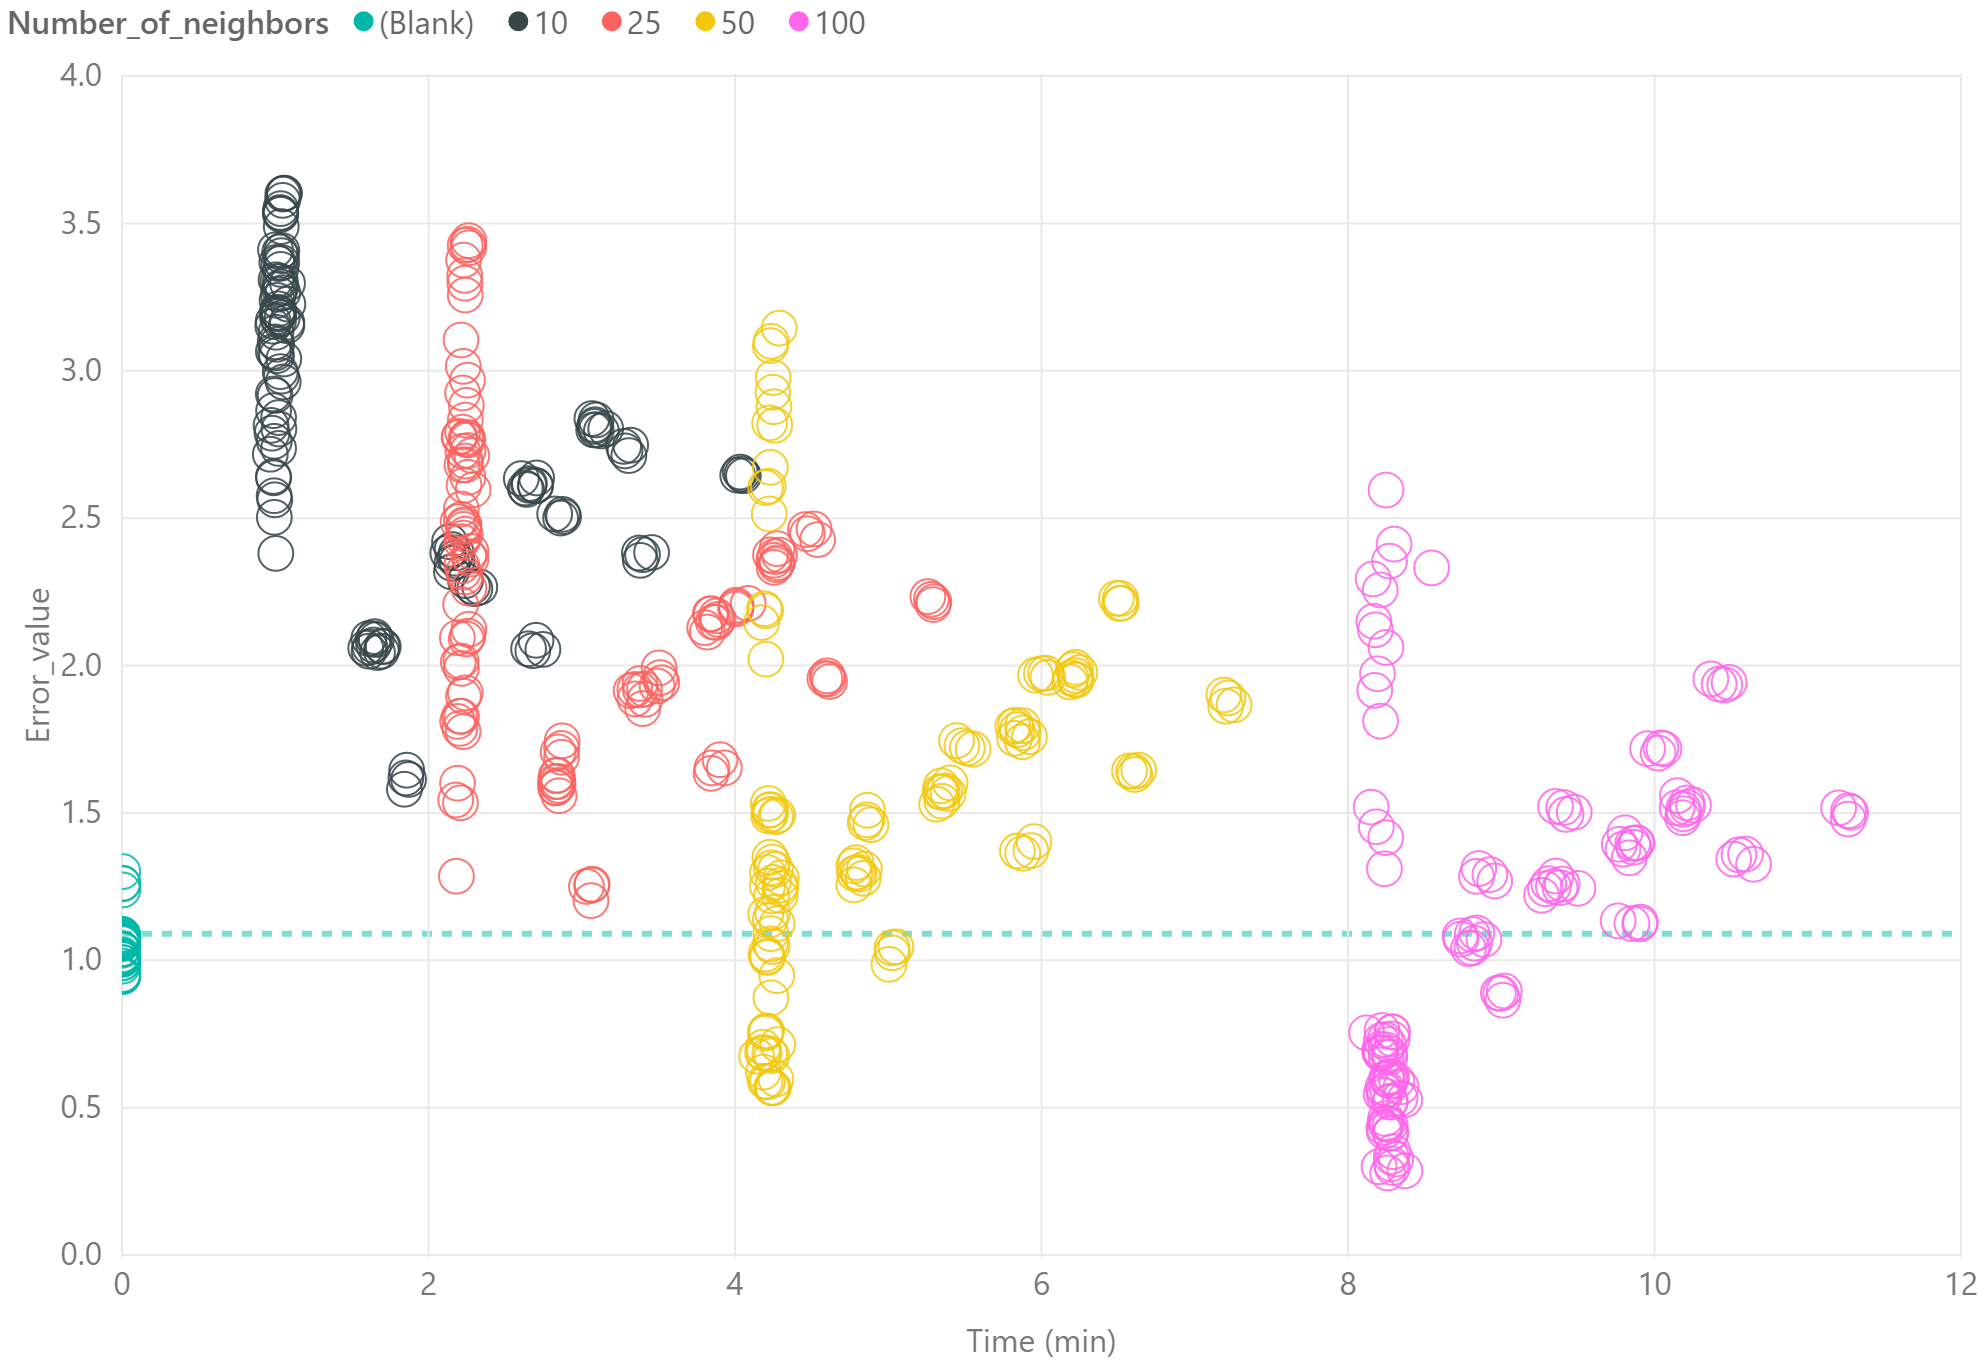
\includegraphics[width=0.60\linewidth]{../Results/Netflix/Plots/Time_RMSE_by_Neighbors.PNG}}
%     \subfigure[Por medida de similitud]{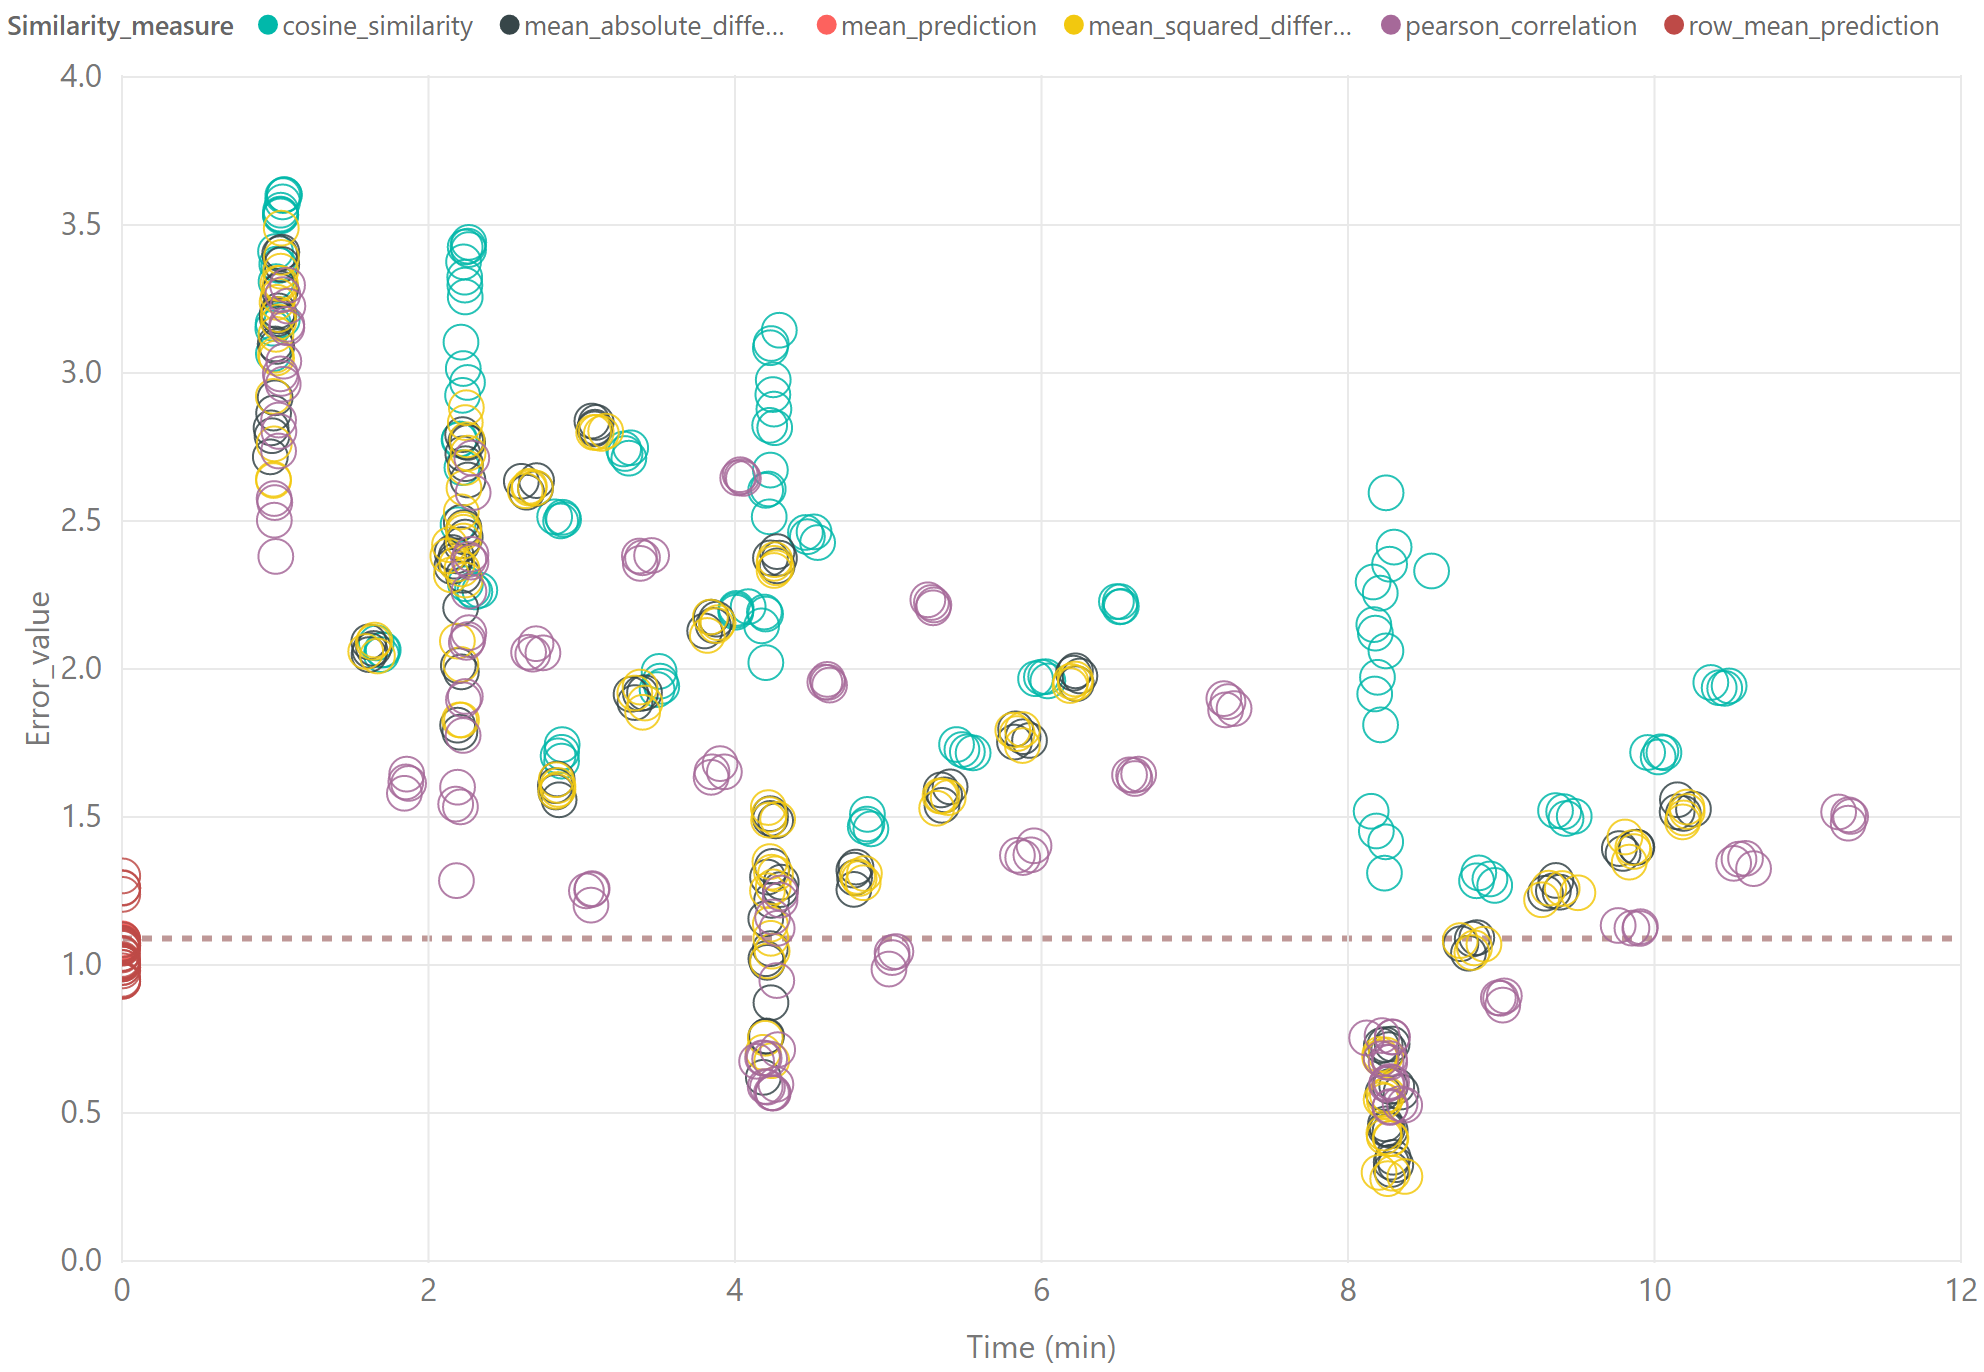
\includegraphics[width=0.60\linewidth]{../Results/Netflix/Plots/Time_RMSE_by_Similarity.PNG}}
%     \subfigure[Por porcentaje de conjunto de entrenamiento]{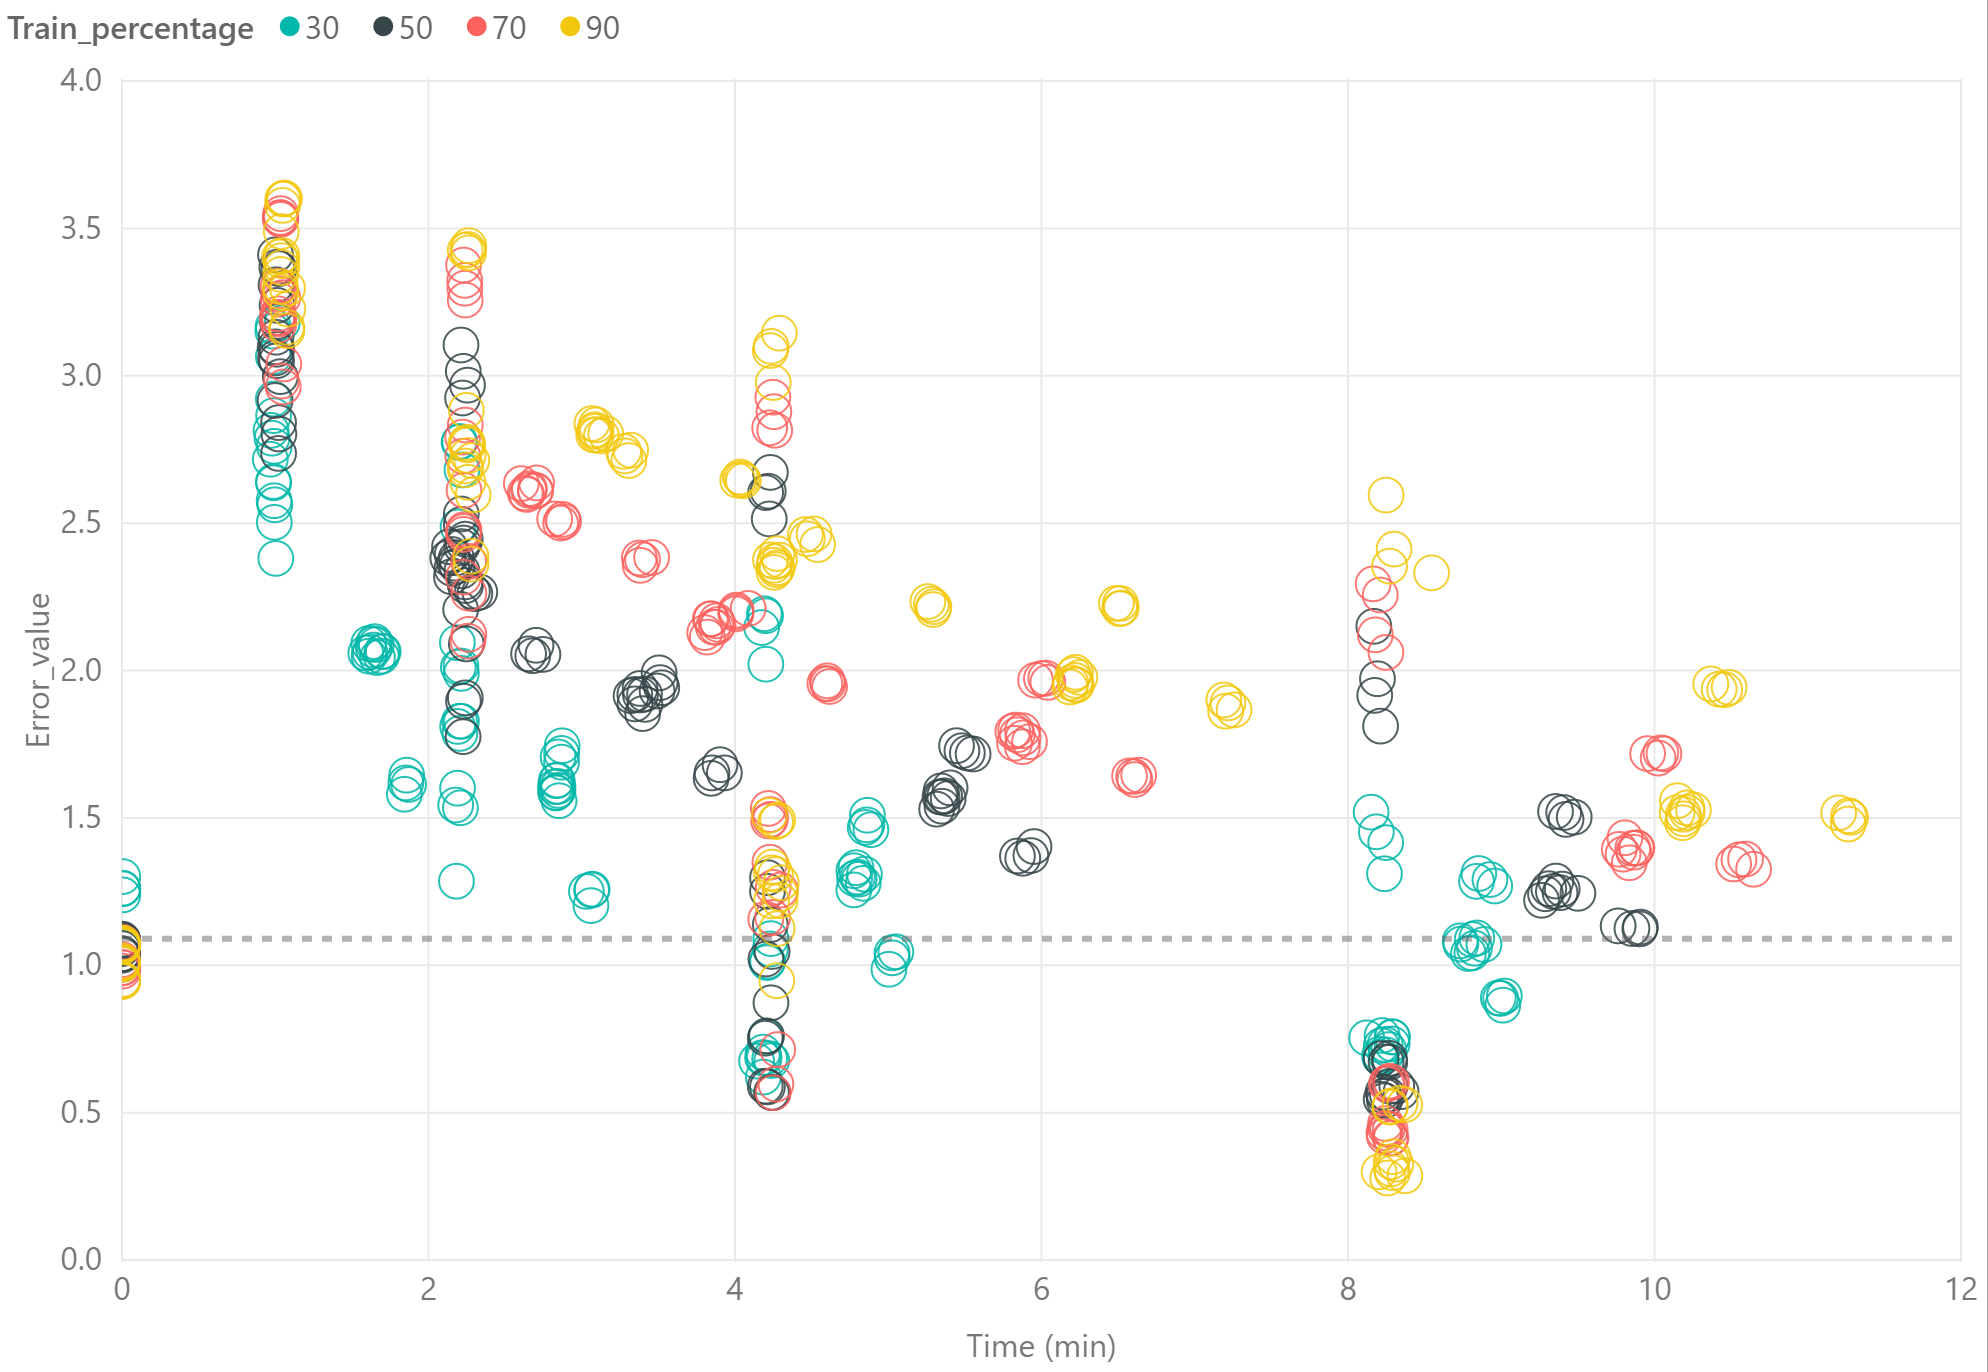
\includegraphics[width=0.60\linewidth]{../Results/Netflix/Plots/Time_RMSE_by_Train.PNG}}
%     \caption{Métodos basados en similitud: Tiempo vs RMSE}\label{fig:Time_RMSE}
% \end{figure}


% \begin{figure}[htb]
%     \centering
%
%     \subfigure[Basado en usuarios, por número de vecinos]{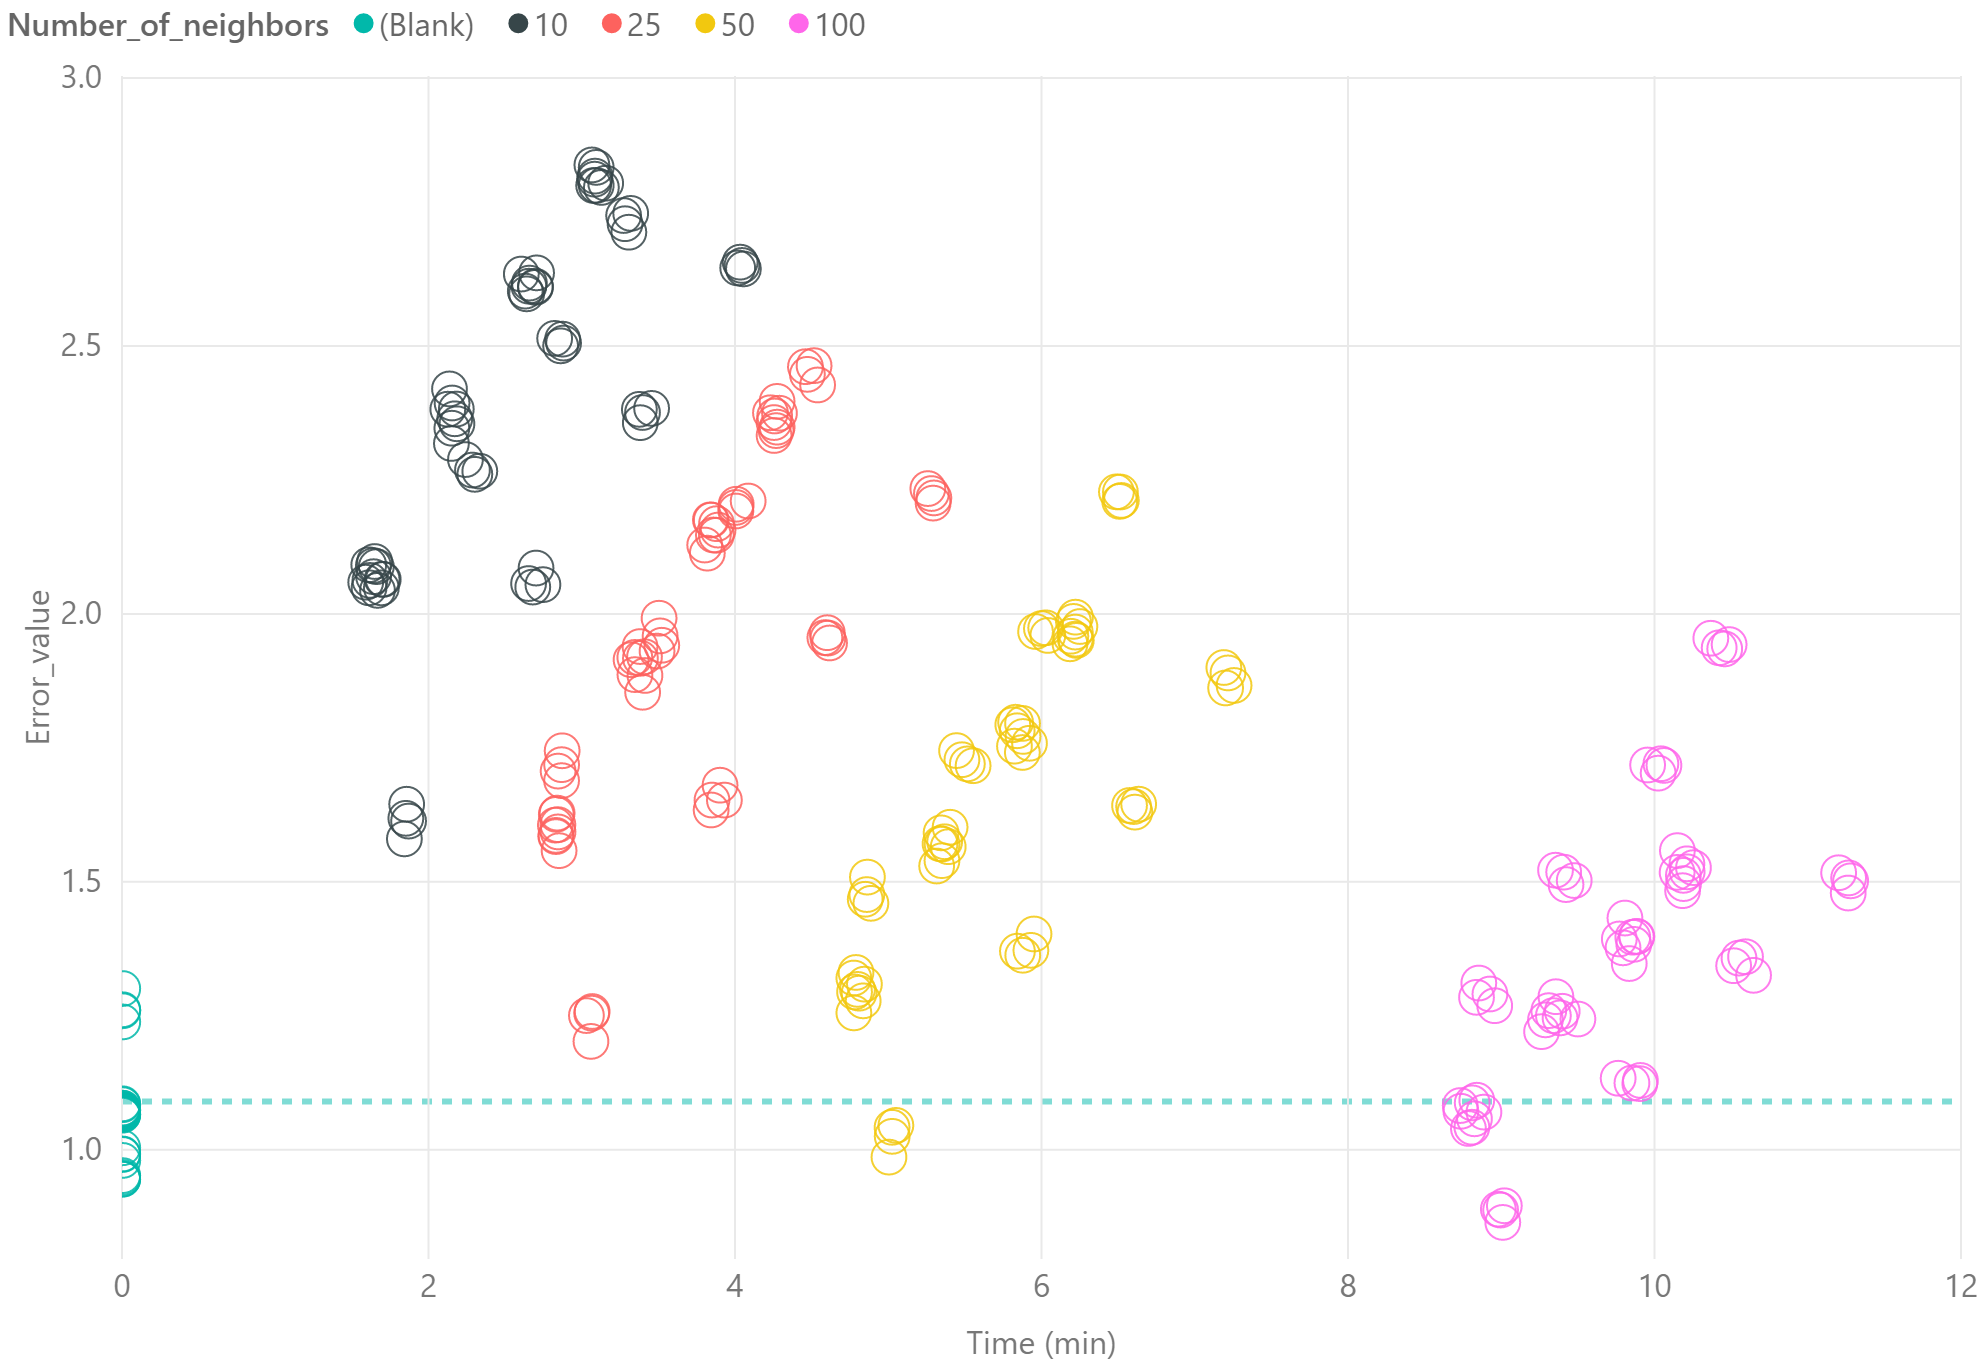
\includegraphics[width=0.48\linewidth]{../Results/Netflix/Plots/UserBased_Time_RMSE_by_Neighbors.PNG}}
%     \subfigure[Basado en películas, por número de vecinos]{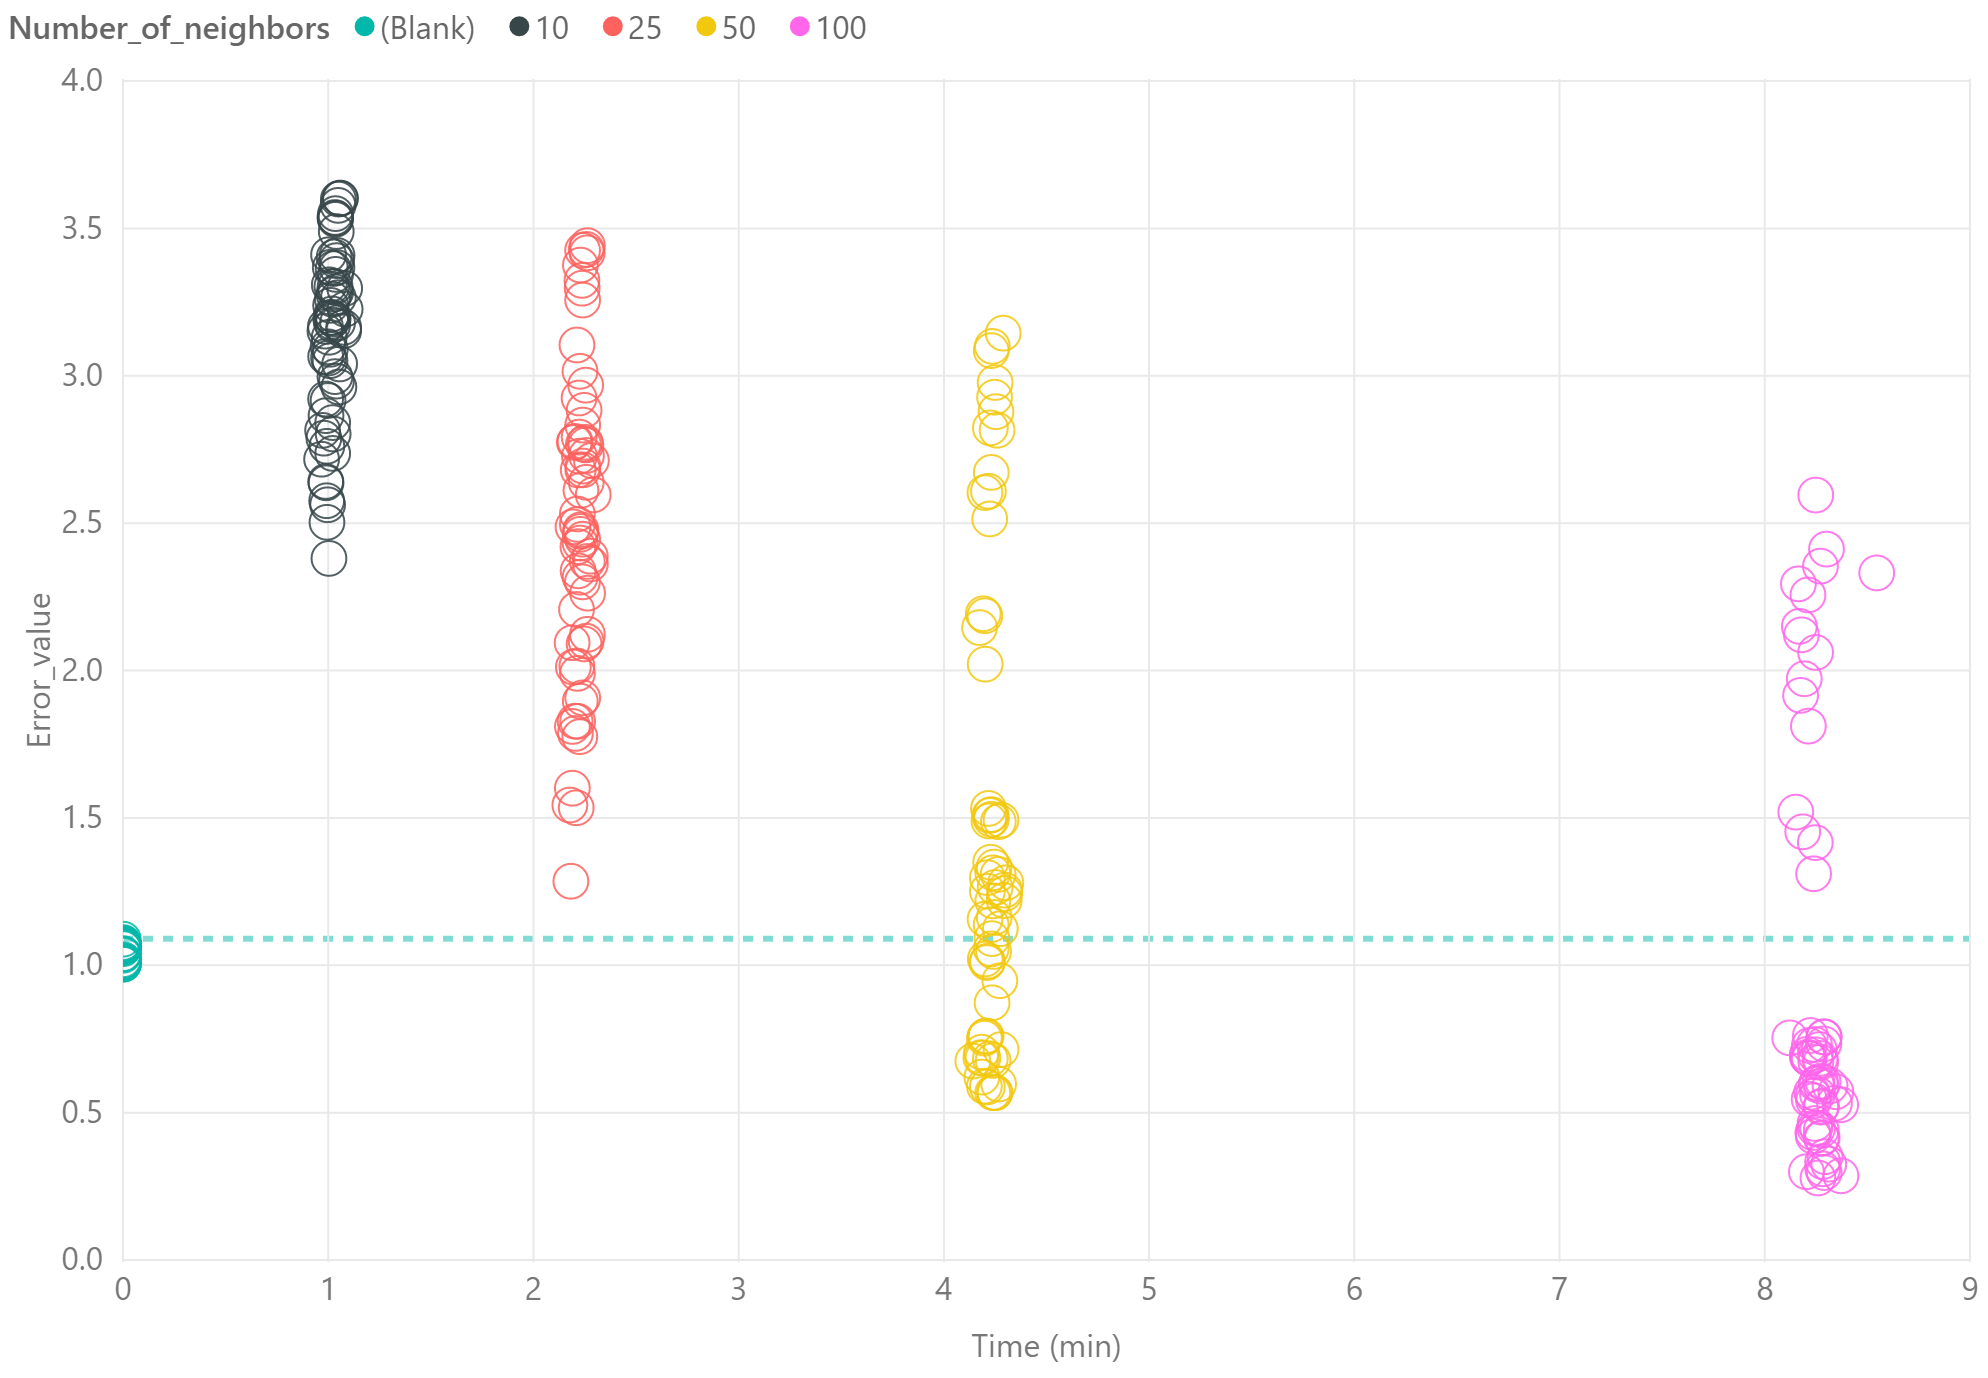
\includegraphics[width=0.48\linewidth]{../Results/Netflix/Plots/ItemBased_Time_RMSE_by_Neighbors.PNG}}
%
%     \subfigure[Basado en usuarios, por medida de similitud]{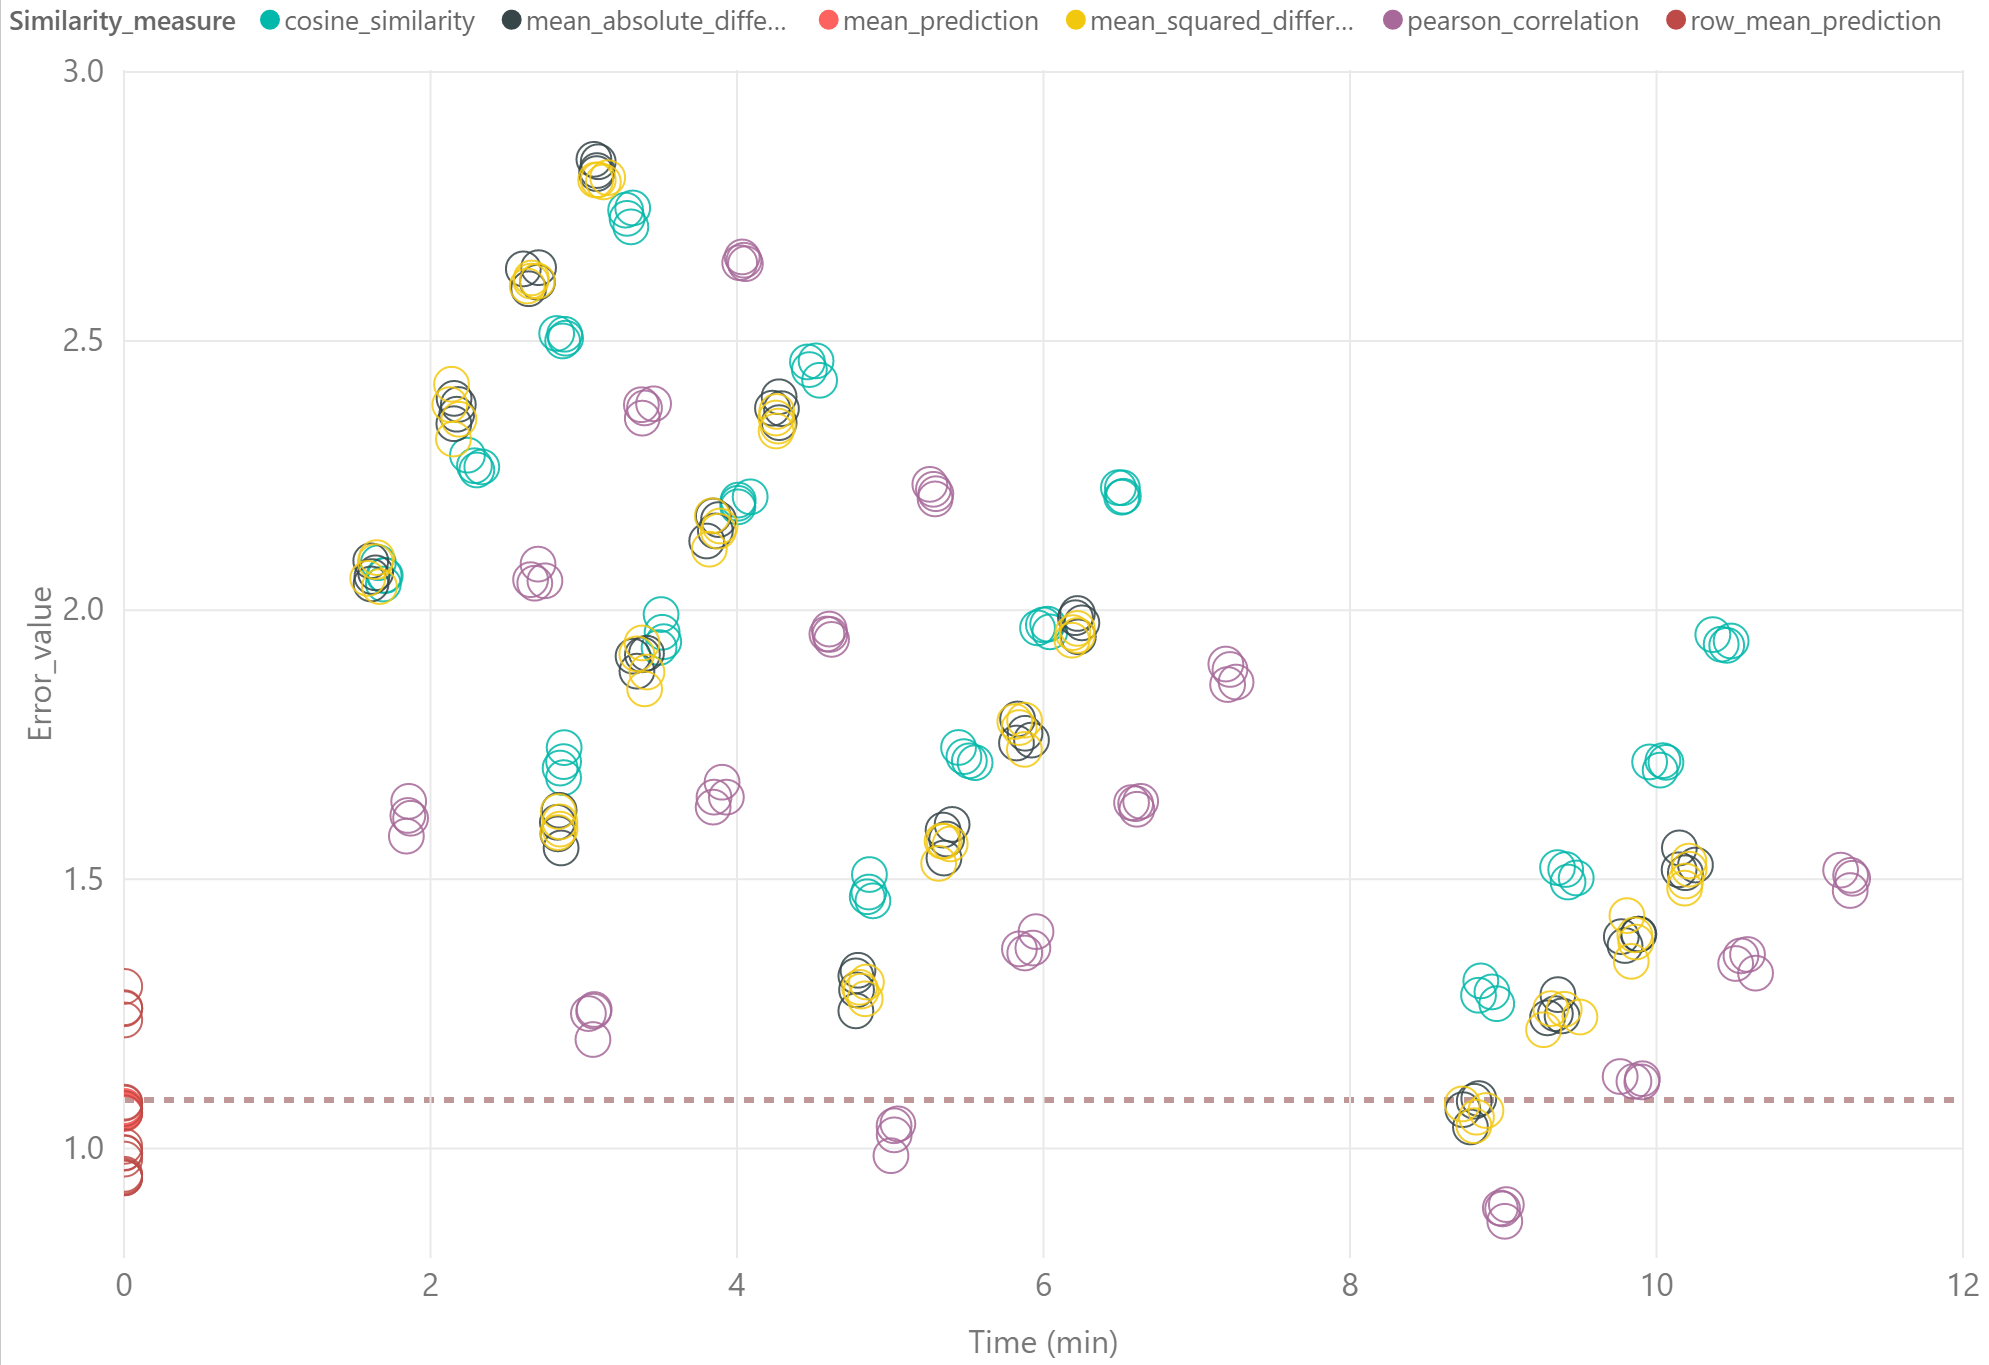
\includegraphics[width=0.48\linewidth]{../Results/Netflix/Plots/UserBased_Time_RMSE_by_Similarity.PNG}}
%     \subfigure[Basado en películas, por medida de similitud]{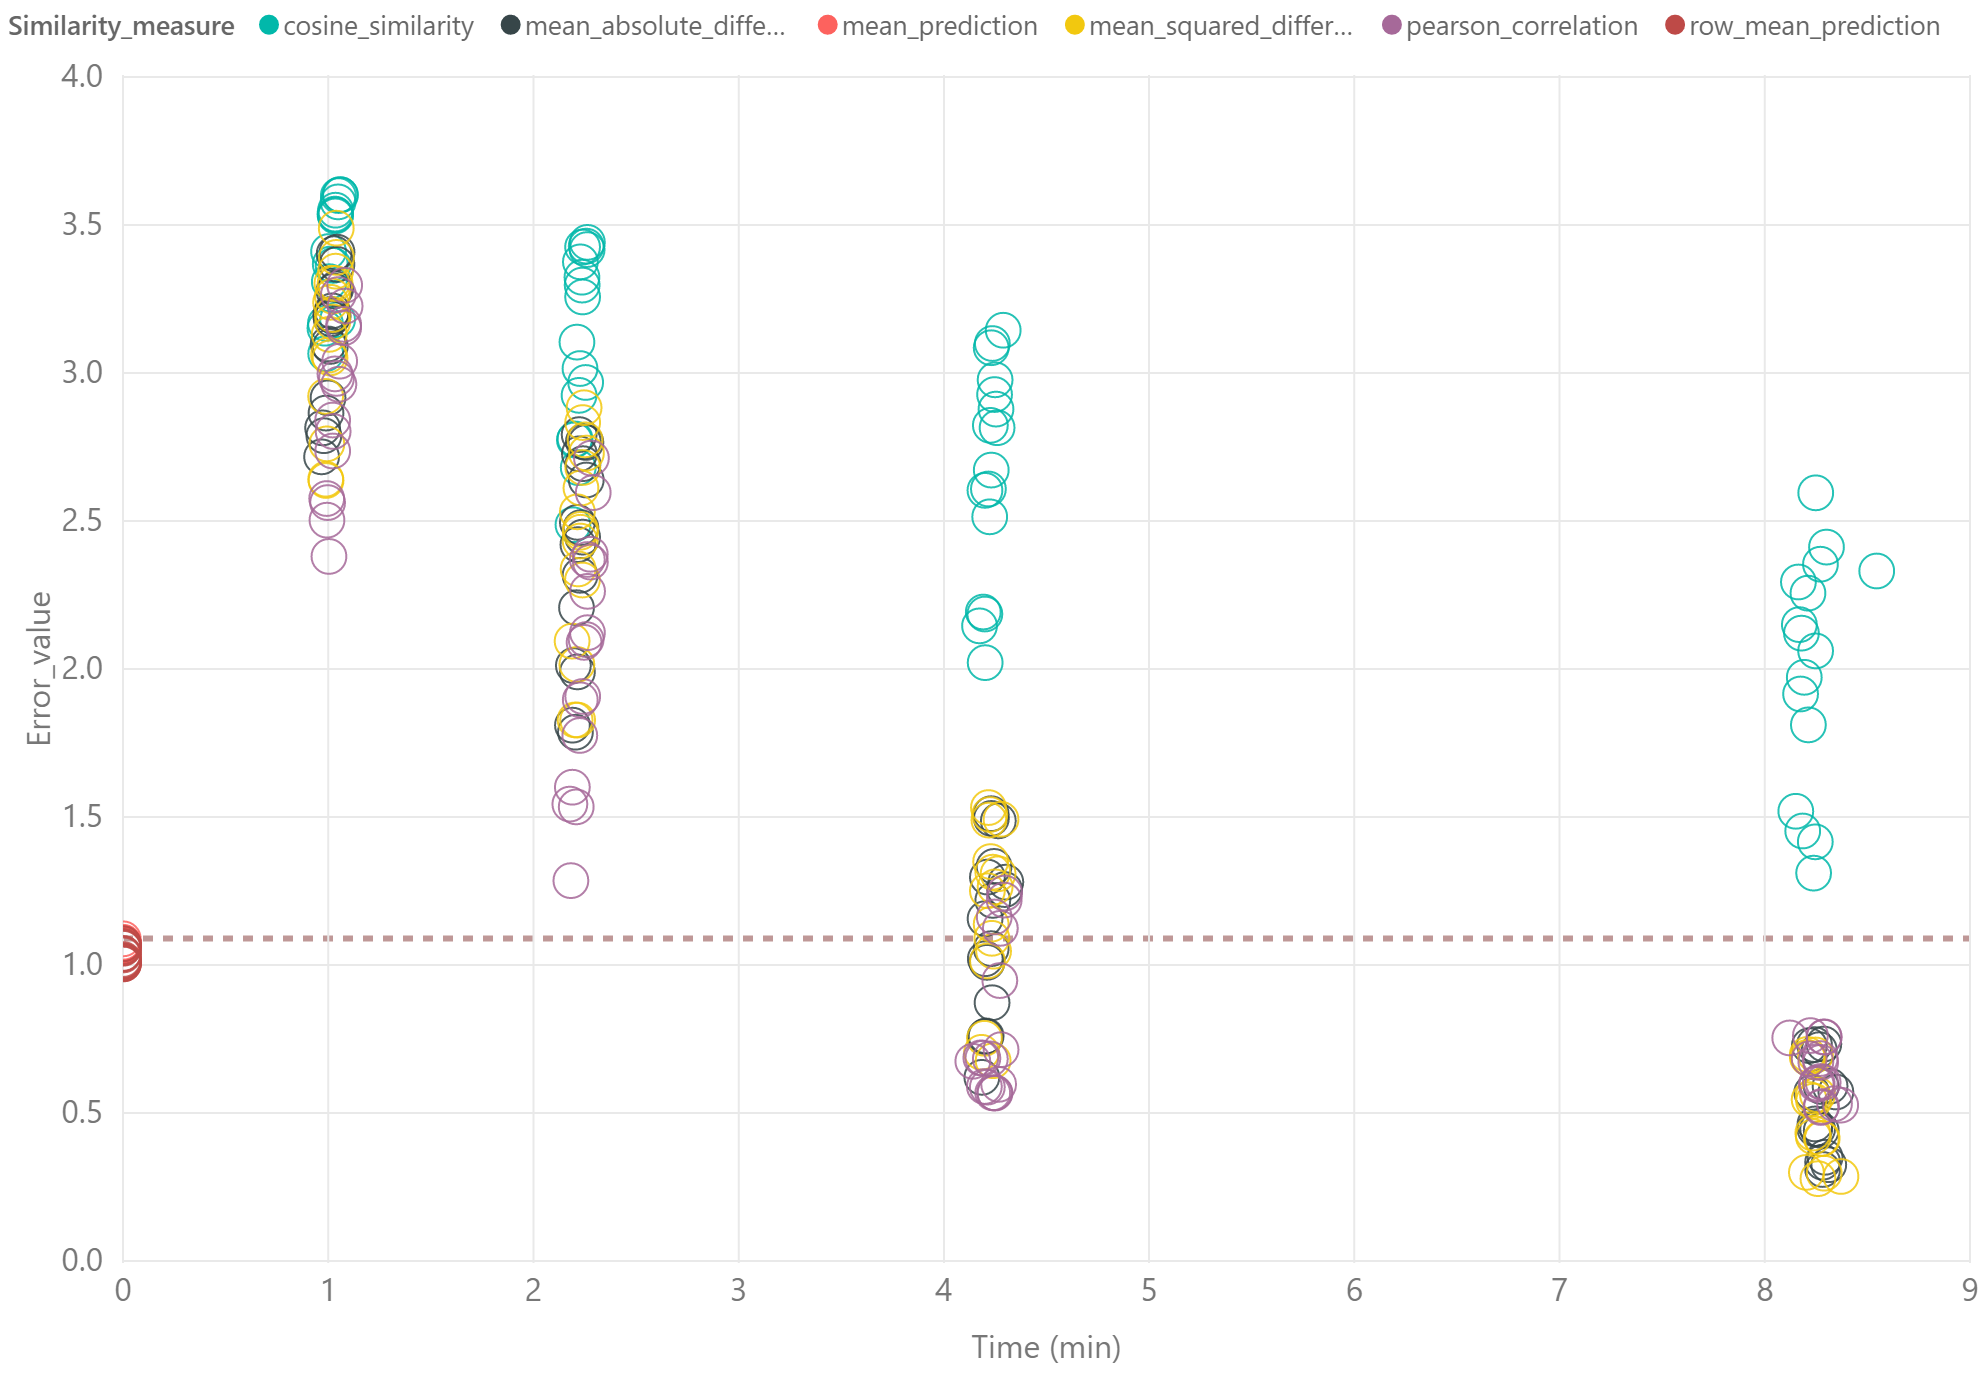
\includegraphics[width=0.48\linewidth]{../Results/Netflix/Plots/ItemBased_Time_RMSE_by_Similarity.PNG}}
%
%     \subfigure[Basado en usuarios, por porcentaje de conjunto de entrenamiento]{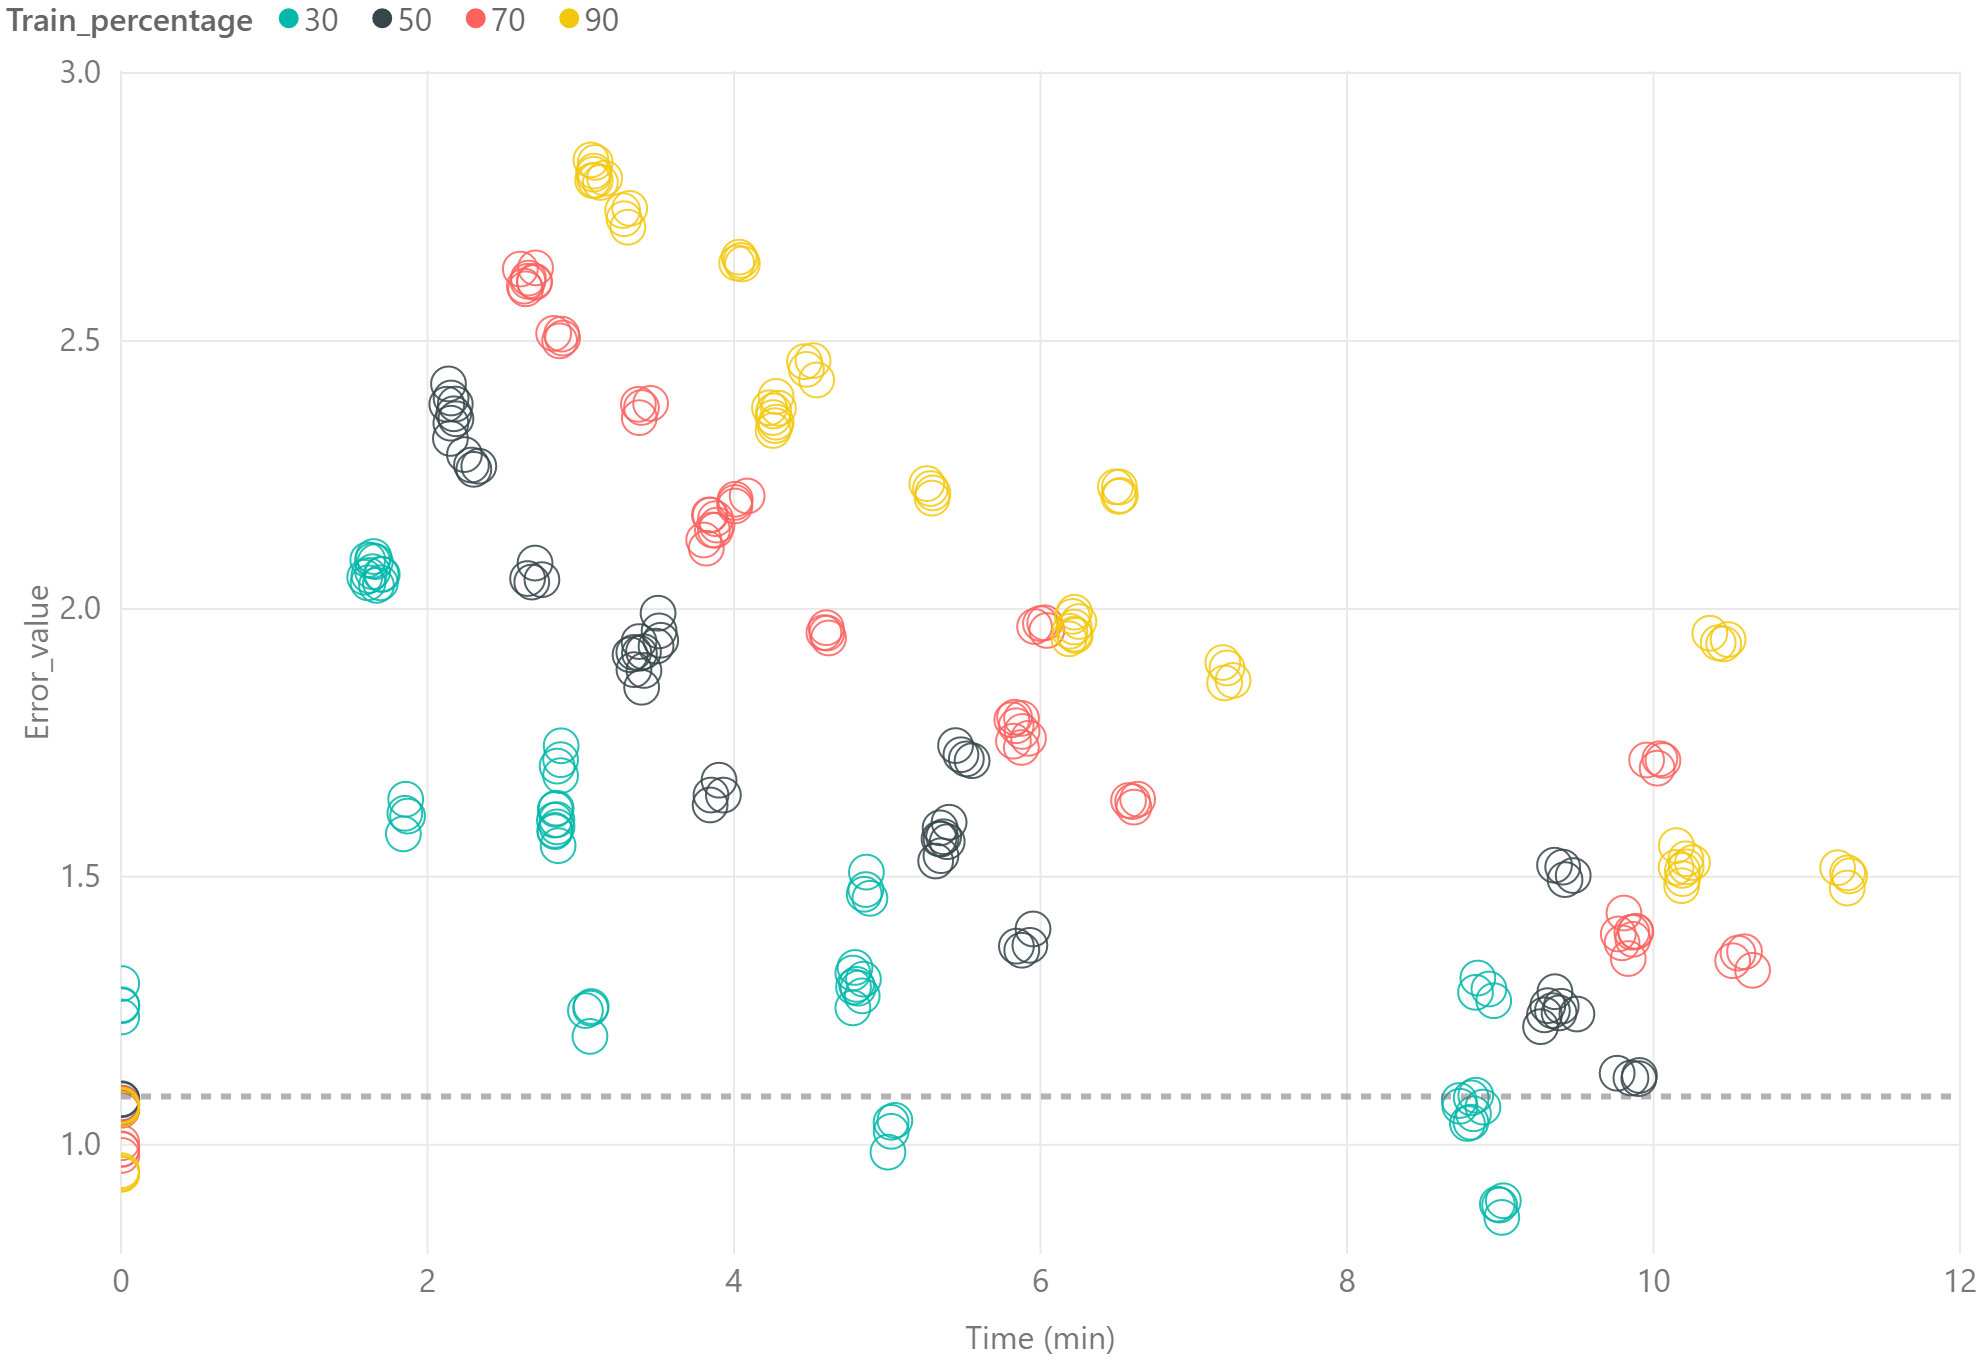
\includegraphics[width=0.48\linewidth]{../Results/Netflix/Plots/UserBased_Time_RMSE_by_Train.PNG}}
%     \subfigure[Basado en películas, por porcentaje de conjunto de entrenamiento]{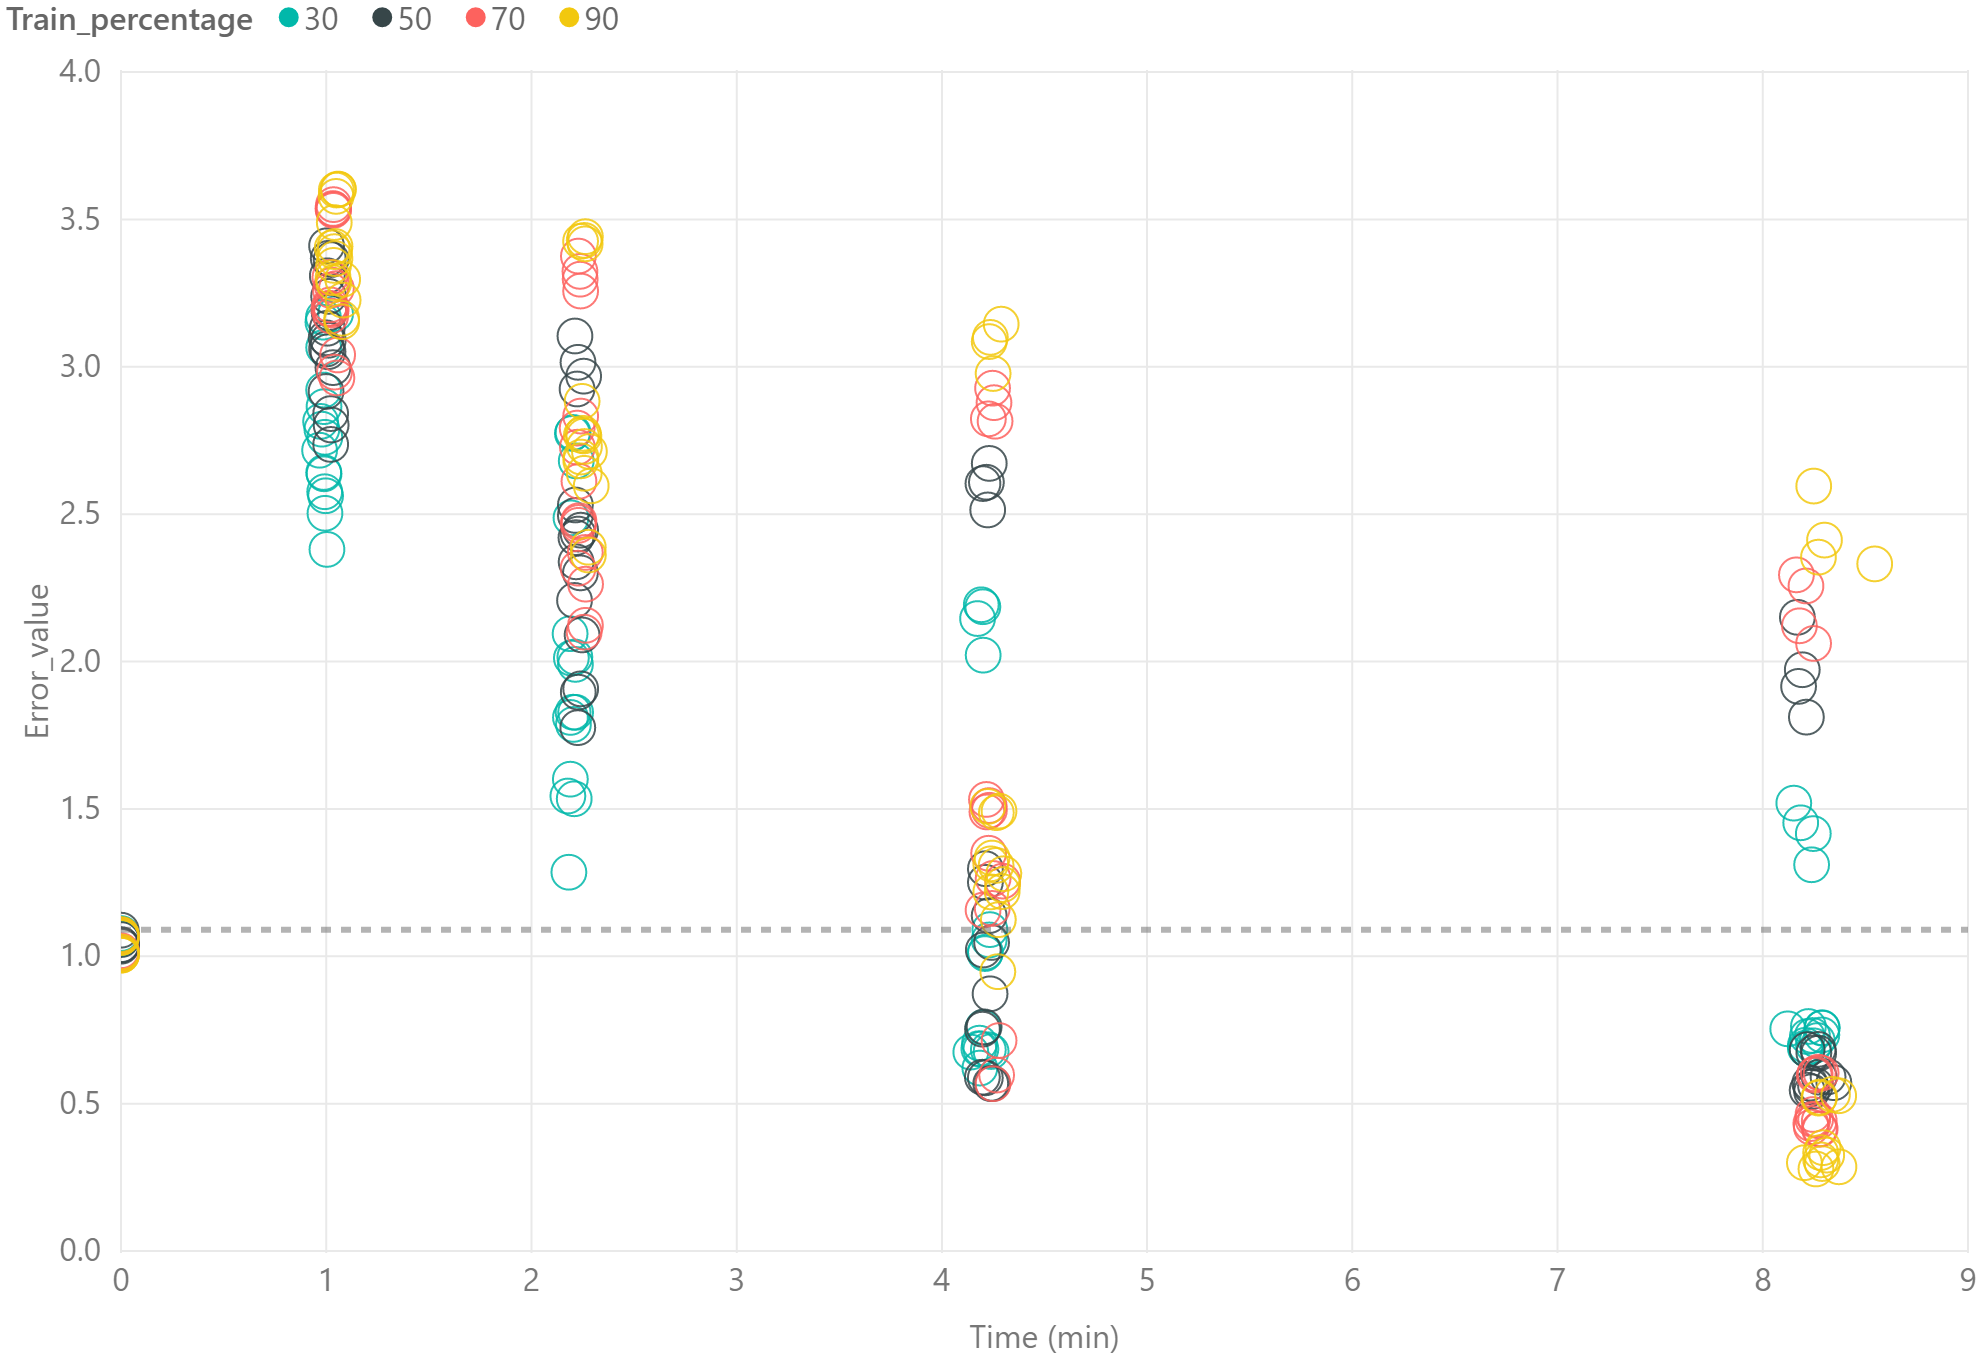
\includegraphics[width=0.48\linewidth]{../Results/Netflix/Plots/ItemBased_Time_RMSE_by_Train.PNG}}
%
%     \caption{Métodos basados en similitud: Tiempo vs RMSE}\label{fig:resultados_similitud}
% \end{figure}

